
\documentclass[10pt]{article}
\usepackage{graphicx}
\usepackage{hyperref}
\usepackage[ngerman]{babel}
\usepackage{siunitx}
\sisetup{
  locale = DE ,
  per-mode = symbol  % whether it should print "/" or "^-1"
}

\usepackage[margin=2.1cm]{geometry}
\usepackage[utf8]{inputenc}
\usepackage{multicol}
\usepackage{nicefrac}
\usepackage{todonotes}
\usepackage{amsmath}
\usepackage{amssymb}
\DeclareMathOperator{\sign}{sign}
\usepackage{wrapfig}
% \usepackage{pdflscape}
% \usepackage{pdfpages}
% \usepackage{epstopdf}
% \epstopdfDeclareGraphicsRule{.tiff}{png}{.png}{convert -density 180 #1 \OutputFile}
% \AppendGraphicsExtensions{.tiff}


\author{Felix Ganz\thanks{Projektgruppe 03 in der Lehrveranstaltung \glqq Autonomes Fahren\grqq\ an der \emph{TUHH} und der \emph{UHH}}\and Nico Albers\footnotemark[1] \and Tim Hansen\footnotemark[1]\and Timo Kias\footnotemark[1]}
\title{Abgabe 2: \emph{Abstandsregler}}
\begin{document}

\maketitle
\tableofcontents

\section{Bilderkennung}
Bei der Bilderkennung haben wir zunächst mit gängigen bereits implementierten Bilderkennungsalgorithmen versucht, ein vorausfahrendes Fahrzeug im Bild der Pi Kamera zu erkennen und ein Rechteck um das gefundene Fahrzeug zu legen.
Da dieser Ansatz besonders bei Kurvenfahrten Fehleranfällig war, haben wir im Folgenden einen anderen Ansatz zur Erkennung des vorausfahrenden Fahrzeugs verfolgt.

Für unseren Ansatz der Bilderkennung haben wir uns überlegt, welche markanten Merkmale das vorausfahrenden Autos hat, um dieses anstelle des gesamten Fahrzeugs im Bild suchen zu lassen.
Unter der Annahme, dass das zu folgende Auto von gleicher Bauart wie unser eigenes Auto ist, haben wir die rot eingefärbten Federn der Hinterradaufhängung als passendes Merkmal für unsere Bilderkennung identifiziert.
Hierzu sei kurz erwähnt, dass wir für einen allgemeineren Ansatz(bspw ein vorausfahrendes Fahrzeug mit anderem Aufbau) unsere Methode durch hinzufügen von erkennbaren Merkmalen entsprechend verwendet werden kann.

Da dieses Merkmal grundsätzlich über sein Farbspektrum der entsprechenden Pixel identifizierbar ist und prinzipiell formunabhängig ist, hielten wir diesen Ansatz für vielversprechend. Ein weiterer Vorteil dieser Idee ist, dass wir zwei Federn identifizieren können, was später im Zusammenhang mit der Abstandsreglung ein entscheidender Faktor sei wird.

Für die Identifikation der roten Federn haben wir das Farbspektrum der Pixel untersucht und dieses nach ihren HSV-Koordinaten mit Hilfe einer Maske gefiltert, wobei HSV hierbei für Hue, Saturation und Value steht.
Dies bietet eine gute Möglichkeit passende Ober- und Untergrenzen von möglichen Koordinaten zu definieren, mit der wir die bereits erwähnte Maske bilden, um die Pixel nach ihren Farbspektrum zu filtern.
Über die H Koordinate kann dabei der Farbton rot relativ direkt benannt werden.
Über die S- und V-Koordinaten konnten wir Farbintensität und Helligkeit einstellen.
Mit der HSV-Maske können wir das Bild in eine binäre Darstellung überführen, in der Pixel mit HSV-Werten innerhalb der definierten Grenzen als wei"se Pixel und Pixel mit Werten außerhalb der Grenzen als schwarze Pixel dargestellt werden.
Mit dieser klaren Abgrenzung von roten zu andersfarbigen Pixeln, haben wir eine Reihe von Regeln erstellt, mit der gefundene rote (nun weis"e) Bereiche als Federn identifiziert werden konnten.
Nachdem zwei passende rote Felder gefunden wurden, haben wir jeweils Hüllkreise mit minimalem Radius um diese gezogen, sodass alle identifizierten Punkte innerhalb dieser Hülle liegen.
Mit dieser nun konkreten Geometrie der gefundenen Federn waren wir in der Lage zunächst die Mittelpunkte und daraufhin den Abstand zwischen diesen in Pixelkoordinaten zu identifizieren.
\todo[inline]{angaben weiterer Verfeinerungen der Grundidee Vorverarbeitung des Kamerabildes eventuell  einige der Regeln. Hier könnte auch ein Beispielbild kommen, welches [...]}

\section{Abstandsregelung}\label{sec:Abstandsreglung}
Im Folgenden stellen wir unsere Überlegungen für das Problem der Abstandsregelung dar.
Bei der Betrachtung dieser Regelungsaufgabe wurde schnell klar, dass das grundlegende Problem darin besteht, dass unsere Bilderkennung Information in Pixelkoordinaten liefert und dass diese lediglich einen zweidimensionalen Raum bilden.
Nach einiger Recherche zu möglichen Rücktransformationen von zweidimensionalen Pixelkoordinaten zu dreidimensionalen Weltkoordinaten war die Problematik dieser Aufgabenstellung um so deutlicher.
Ohne zusätzliche Informationen darüber was in dem Bild zu sehen ist, sind direkte analytische Lösungen nicht vorhanden und auch mit Informationen über bekannte Geometrien im Bild sind weitere Annahmen nötig, um auf eine eindeutige Tiefe in Weltkoordinaten Rückschlüsse zu führen.
Mit der Annahme, dass das Zielobjekt auf einer ebenen Fläche fährt und das die identifizierte Punkte parallel zu dieser Fläche liegen, ist eine Rückrechnung der Pixelkoordinaten in Weltkoordinaten mit Hilfe der identifizierten Federn aus der Bilderkennung und deren Abstand zueinander zumindest für die Pixel möglich, die das Auto darstellen.
Damit auch der Abstand des Hecks zu der Kamera des folgenden Autos.
Die Überlegung dazu beruht auf dem Schema dargestellt in Abb.
\ref{fig:reifenradius}.
Bei bekannter Größe des Objekts $H$ in Weltkoordinaten und $h$ in Bildkoordinaten sowie ermitteltem Fokus $f$ kann der Abstand $z$ wie folgt berechnet werden.
\begin{eqnarray}
z = \frac{fh}{H}
\end{eqnarray}
Unter Verwendung dieses einfachen Zusammenhangs könnte man nun aus den ermittelten Abständen der Federn aus der Bilderkennung und bekanntem Abstand der Federn am realen Auto den Abstand von Kamera zu vorausfahrendem Auto ermitteln und dann über eine weitere Transformation von Kamerakoordinatensystem zu einem autofesten Koordinatensystem den Abstand zwischen Front und Heck der Fahrzeuge ermitteln.\\
\begin{figure}[hbtp]
    \centering
    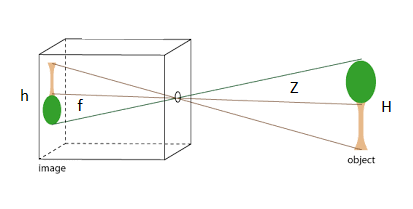
\includegraphics[width=0.5\textwidth]{Pinholeobject_label}
    \caption{Schematische Darstellung der Tiefeninformation bei bekannter Geometrie}
    % \vspace{-20pt}
    \label{fig:reifenradius}
\end{figure}
Stattdessen haben wir uns für eine Lösung entschieden, die auch als \textit{vision based control} bekannt ist. Bei dieser Art der Abstandsregelung haben wir auf die Transformation von Pixelkoordinatensystem zu Weltkoordinatensystem verzichtet und haben die nötigen Berechnung zur Reglung komplett im Pixelkoordinatensystem durchgeführt. Unsere Reglerstruktur besteht aus zwei entkoppelten Reglern $C_u$ und $C_{\gamma}$, bei dem der Regler $C_u$ für den Abstand in Tiefenrichtung und der Regler $C_{\gamma}$ für den Abstand in Breitenrichtung beides bezüglich Weltkoordinatensystem verantwortlich ist. Da wir jedoch keine Transformation zum Weltkoordinatensystem durchführen, haben wir die Informationen aus der Bilderkennung in entsprechende Fehlergrößen $e_u$ und $e_{\gamma}$ überführt, die dann durch den entsprechenden Regler in eine Motoransteuerung $u$ und einen Lenkwinkel $\gamma$ umgerechnet werden.

\begin{eqnarray}
u = C_u(e_u) \\
\gamma = C_{\gamma}(e_{\gamma})
\end{eqnarray}

Den benötigten Fehlergrößen liegen folgende Überlegungen zu Grunde:\\
Für den Abstandsfehler $e_u$ geben wir dem System ein Referenzbild, aufgenommen mit der Pi Kamera vor, in dem das vorausfahrende Auto im gewünschten Abstand vor dem Verfolger steht. Der über die Bilderkennung ermittelte Abstand der Federn in Pixelkoordinaten dient im folgenden als Referenzgröße $d_{f,r}$. Dieser kann bei Bedarf auch "hart" in Pixelgrößen im System hinterlegt werden. Im Laufe der Fahrt wird nun jedes eingehende Bild analysiert und ein aktueller Abstand $d_{f,a}$ mit der Referenzgröße verglichen um den Abstandsfehler
\begin{eqnarray}
e_u = d_{f,r} -d_{f,a}
\end{eqnarray}
zu bilden. Vergrößert das vorausfahrende Fahrzeug den Abstand zum Verfolger wird der erkannte Abstand $ d_{f,a} $ kleiner und die Fehlergröße positiv. Andersherum wird die Fehlergröße negativ. Im Falle eines negativen Fehlers haben wir den Motorinput zu Null gesetzt, damit der Verfolger bremst und nicht mit negativer Motoransteuerung rückwärts fährt\\
Im Falle des Lenkfehlers $e_{\gamma}$ wird kein Referenzbild benötigt. Hier wird zu jedem Zeitpunkt der Mittelpunkt $M=[M_x, M_y]$ der Verbindungslinie zwischen der in der Bilderkennung ermittelten linken und rechten Feder ermittelt. Daraufhin bilden wir den horizontalen Abstand bezüglich der Bildmittellinie $e_{\gamma}$
\begin{eqnarray}
e_{\gamma} = x_0 - M_x.
\end{eqnarray}
Die horizontale Koordinate der Bildmittellinie $x_0$ ist aus der Kamerakalibrierung als zentraler Punkt der Bildebene bekannt.\\
In beiden Fällen haben wir den eingehenden Fehler mit dem im allgemeinen am größten zu erwartenden Fehler skaliert, um den Eingang des Reglers auf dem Bereich [-1,1] zu normieren. Durch diesen Schritt ist es zum einen klarer die Reglerparameter zu wählen und zum anderen ist eine Abbildung auf den jeweils möglichen Ausgangsbereich für Motoransteuerung und Lenkwinkel besser möglich.\\
Als erste Implementierung haben wir die beiden Regler als Proportionalregler ausgelegt. Prinzipiell können in dem oben beschriebenen Rahmen aber auch weitere Reglerfunktionen angewendet werden.\\


\section{Performance und Parameteroptimierung}
Für diese Abgabe haben wir uns auf die oben beschriebene Reglerstruktur unter Verwendung eines Proportionalreglers beschränkt, da wir nach ersten Testläufen mit einem aufgebockten Fahrzeug erkannten, dass unsere Regler zwar das gewünschte Verhalten zeigen, aber die Umsetzung nicht in Echtzeit erfolgte. Um die Rechenleistung zu erhöhen, haben wir das analysierte Bild verkleinert, indem wir nur im Abstand von unseren oben genanten Referenzpunkten gesucht haben. Die zugrundeliegende Idee hierbei ist, dass das vorausfahrende Auto sich selbst in Kurven nicht sprunghaft aus unserem Bild entfernt und der betrachtete Ausschnitt mit jedem folgenden Bild in Richtung des Autos versetzt wird. [TBA]\\
Wie in Kap. \ref{sec:Abstandsreglung} beschrieben, verwenden wir die beiden Regler $C_u$ und $C_{\gamma}$.\\
Der Regler für den Lenkeinschlag $C_{\gamma}(e_{\gamma})$ hat zum Zeitpunkt der Abgabe die folgende interne Struktur
\begin{eqnarray}
C_{\gamma}(e_{\gamma}) = \begin{cases} k_{\gamma}e_{\gamma}\gamma_{max} & |e_{\gamma}| \leq 1 \\
                                        -\sign (e_{\gamma})\gamma_{max} &  |e_{\gamma}| > 1
\end{cases}
\end{eqnarray}
Mit $k_{\gamma}$ einer proportionalen Verstärkung und $\gamma_{max}$ dem maximal möglichen Lenkeinschlag des Fahrzeugs. Die Fallunterscheidung um den Wert eins ergibt sich durch eine Skalierung des Fehlerwertes auf einen Toleranzabstand um die Mittellinie des Bildes, welche eingeführt wurde um einem Herausfahren des zu folgenden Fahrzeugs aus dem Bild der Py Kamera durch einen maximalen Lenkeinschlag entgegen zu wirken.\\
Der Regler für den Abstandsregler $C_{u}$ hat zum Zeitpunkt der Abgabe die folgende interne Struktur
\begin{eqnarray}
C_{u}(e_{u}) = \begin{cases} 0 & e_{u} \leq 0 \\
\max (fk_{u}e_{u}u_{max},u_{min}) &  e_{u} > 0
\end{cases}\\
\text{mit } f(\gamma)=1-\frac{\gamma}{\gamma_{max}}x
\end{eqnarray}
Hierbei sind $k_{u}$ eine proportionale Verstärkung, $\gamma_{max}$, $u_{max}$ die jeweils maximalen Ansteuerungen von Motor und Lenkeinschlag und $u_{min}$ ein minimaler Motoreingang, der nötig ist um Haftreibung zu überwinden. Die zusätzliche Skalierung $f(\gamma)$ modelliert eine Abhängigkeit des erkannten Abstandes der Federn und darüber des vom Regler erzeugten Motoreingangs zum Gierwinkel des vorausfahrenden Fahrzeugs als proportionale Dämpfung des Eingangs $u$. Unsere Reglerstruktur ist in Abb.\ref{fig:struktur} dargestellt.\\
\begin{figure}[hbtp]
    \centering
    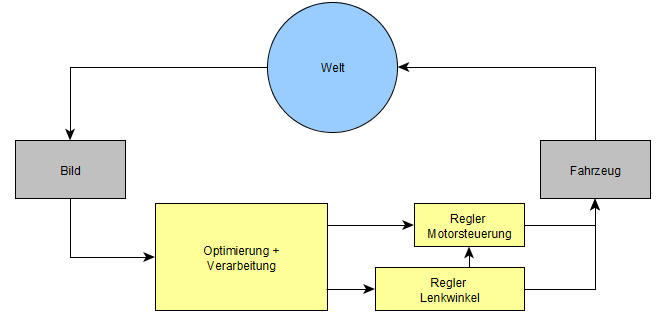
\includegraphics[width=0.5\textwidth]{Autonomes_Fahren_Welt_Regler}
    \caption{Darstellung der Reglerstruktur}
    % \vspace{-20pt}
    \label{fig:struktur}
\end{figure}


\section{Grenzen und Ausblick}
Die oben beschriebene Methode zur Steuerung des Fahrzeug hat gewisse Grenzen.
Das Fahrzeug kann nur folgen.
Falls das vordere Fahrzeug rückwärts fährt, wird es mit unserem Fahrzeug kollidieren.\\
Zu Beginn haben wir die Regler unabhängig voneinander programmiert.
Da der Abstand zwischen den getrackten Punkten in einer Kurve allerdings abnimmt, obwohl das führende Fahrzeug sich nicht in diesem Maße vom folgenden Fahrzeug entfernt, haben wir den eingeschlagenen Winkel als Drosselung einbezogen.
Da wir allerdings auch einen entsprechend starken Winkel einschlagen müssen um die Punkte entsprechend zu tracken, hat dies die Geschwindigkeit reduziert.
Für diese Aufgabe wollten wir allerdings mit möglichst starken Winkeln folgen und haben wir diesen Nachteil daher akzeptiert.


Ein weiterer Aspekt ist das Verhalten des Fahrzeug falls es die Punkte verliert.
Momentan fährt es mit dem letzten bekannten Winkel sowie Geschwindigkeit weiter.
Als mögliche Stabilisierung könnten hierzu bspw.
die Kanten der Kameraaufhängung des führenden Fahrzeugs getrackt werden und bei Trackingverlust mit mindestens einem bekannten Punkt der andere Punkt auf der gegenüberliegenden Seite der Aufhängung angenommen werden.

Zusammenfassend lässt sich sagen, dass unsere Regelung bei wechselnden niedrigen bis mittleren Geschwindigkeiten auch mit Kurven recht sicher ausgeführt wird.
Als mögliche Optimierungen sehen wir insbesondere die Bilderkennung über einen größeren Zeitraum, da wir aktuell immer nur anhand eines Bildes tracken.
Hierbei muss allerdings immer die Rechenleistung des Pi beachtet werden.
Auch mit komplexeren Reglern können wir voraussichtlich insbesondere die Geschwindigkeit erhöhen.

\section{Teamarbeit}
Dadurch, dass alle Aufgaben von unserem Team gemeinsam gelöst wurden, gab es keine direkte Aufteilung der einzelnen Aufgaben. Wir haben Ideen in Teamarbeit entwickelt und gemeinsam vorangetrieben.

\end{document}
